\documentclass{article}

\usepackage[utf8]{inputenc}
\usepackage[portuguese]{babel}
\usepackage{blindtext}
\usepackage{graphicx}
\usepackage{amsmath}
\usepackage{float}
\usepackage{caption}
\usepackage[compact]{titlesec}
\usepackage{multicol}
\usepackage[a4paper, total={7.5in, 10in}]{geometry}
\usepackage[font=scriptsize,labelfont=bf]{caption}
\usepackage{listings}
\usepackage{color}

\definecolor{codegreen}{rgb}{0,0.6,0}
\definecolor{codegray}{rgb}{0.5,0.5,0.5}
\definecolor{codepurple}{rgb}{0.58,0,0.82}
\definecolor{backcolour}{rgb}{0.95,0.95,0.92}
 
\lstdefinestyle{mystyle}{
    backgroundcolor=\color{backcolour},   
    commentstyle=\color{codegreen},
    keywordstyle=\color{magenta},
    numberstyle=\tiny\color{codegray},
    stringstyle=\color{codepurple},
    basicstyle=\footnotesize,
    breakatwhitespace=false,         
    breaklines=true,                 
    captionpos=b,                    
    keepspaces=true,                 
    numbers=left,                    
    numbersep=5pt,                  
    showspaces=false,                
    showstringspaces=false,
    showtabs=false,                  
    tabsize=2
}
 
\lstset{style=mystyle}

\setlength{\columnsep}{1cm}
\setlength{\parindent}{0em}
\titlespacing{\section}{1pt}{*-0.55}{*-0.8}
\begin{document}

\textbf{Relatório de Entrega de Trabalho} \newline
\textbf{Disciplina de Programação Paralela (PP)}\textbf{ - Prof. César De Rose} \newline
\textbf{Alunos:} Rafael Rios e Rodrigo Silveira \newline
\textbf{Exercício:} TPP3: MPI Fases Paralelas (FP)

\begin{multicols*}{2}

\section{Implementação}
O objetivo deste trabalho foi implementar usando a biblioteca MPI um algoritmo seguindo o modelo de fases paralelas para ordenar um vetor de 1000000 de elementos usando bubblesort. Cada processo recebe uma parte igual do vetor e a ordena localmente, verificando se o mesmo está ordenado em relação aos processos vizinhos e, se não está, realizam-se trocas entre seus elementos visando a ordenação do vetor. Os processos seguem a ordem de seus respectivos índices, em uma lista da esquerda para a direita de 0 até o número de processos(np) - 1, a implementação se inicia com cada vetor local sendo criado dentro de seu respectivo processo e recebendo uma parcela de elementos do vetor de tamanho integral proporcional ao número de processos. O vetor é inicializado em ordem decrescente (pior caso) e um vetor auxiliar (vet\_pronto) é usado para armazenar o estado de todos os processos, cada posição corresponde ao índice de um processo, com o valor '1' se o vetor local daquele processo está ordenado, e '0' quando não está. Os vetores são ordenados utilizando o algoritmo bubblesort e compara-se o maior valor do vetor, com o menor valor do vetor do processo a sua direita (menos para o processo de rank 0, que só envia o elemento), se o dado enviado for menor, o vetor está ordenado em relação ao seu vizinho, atualizando a sua posição correspondente em  vet\_pronto para '1'. Através da função MPI\_Bcast, é feita a atualização do vet\_pronto de todos os processos, conferindo se é o fim da execução (todas as posições em '1'). A troca de elementos é realizada através de posições auxiliares nos vetores locais: fixou-se o número de elementos a serem trocados em 1,5\% do total (1000000), cada processo (exceto o 0) envia essa quantidade de seus menores valores para o vizinho à esquerda, o qual recebe e ordena esses elementos com a mesma quantidade de seus maiores valores, devolvendo para o processo que enviou os maiores elementos após essa ordenação. O algoritmo retorna para a etapa de ordenação do vetor completo, sendo assim, todos os processos executam o mesmo código novamente, até que o vetor esteja ordenado.
\section{Dificuldades encontradas}
Encontramos dificuldade para usar corretamente a função MPI\_Bcast, de maneira a manter o sincronismo de vet\_pronto. Outras dificuldades foram: a implementação da inicialização dos vetores localmente, visto que, inicialmente, tentou-se criar um único vetor que deveria ser particionado entre todos os processos, porém essa técnica tornou-se mais complexa do que tínhamos previsto; e a escolha da quantidade ótima de elementos a serem trocados entre os vetores de modo a convergir para a solução desejada de maneira mais rápida.  
\section{Testes}
Foram realizados testes com alocação de 2 nodos exclusivos na máquina grad, executando o código para 16 e 32 processos. Em ambos os casos, os testes foram feitos para diferentes quantidades de elementos sendo trocados entre os processos, visando obter o melhor resultado possível. A primeira execução foi realizada com 0.25\% do tamanho total do vetor (1000000), a cada novo teste, aumentou-se esse valor em 0.25\%, percebendo que após 1.5\% o tempo de execução não aumentava, e para valores muito maiores, o algoritmo sequer convergia para a solução desejada. Ao final dos testes, o melhor resultado obtido foi 553.4 segundos para 16 processos e 358.3 segundos para 32 (HT).
\section{Análise de desempenho}
A versão paralela do algoritmo teve um resultado melhor em comparação com a execução sequencial, obtendo menores tempos de execução, todavia a eficiência ficou abaixo do ideal para ambos os números de processos, atingindo 0.5 de eficiência (D) para 16 processos e 0.4 para 32 (E). O speed-up obtido também foi abaixo do ideal, 8 para 16 processos e 12.4 para 32. Em comparação com o algoritmo de divisão e conquista (D\&C) implementado no trabalho anterior, o resultado do algoritmo de fases paralelas foi muito inferior. Como pode ser visto na Figura 1, as barras A, B e C correspondem à eficiência das três execuções do algoritmo divisão e conquista: implementação ingênua (sem ordenamento local) até 31 processos (HT), implementação com ordenamento local e implementação ingênua sendo executada com mais de 31 processos. Esses resultados demonstram a grande diferença de performance quando comparados aos resultados do algoritmo de ordenação por fases paralelas, devido ao fato do algoritmo desse trabalho não ser projetado para solucionar esse tipo de problema, gastando muito mais tempo ordenando do que realizando a comunicação, de modo que a convergência é lenta.  
\begin{figure}[H]
            \centering
            \vspace{-1.1em}
            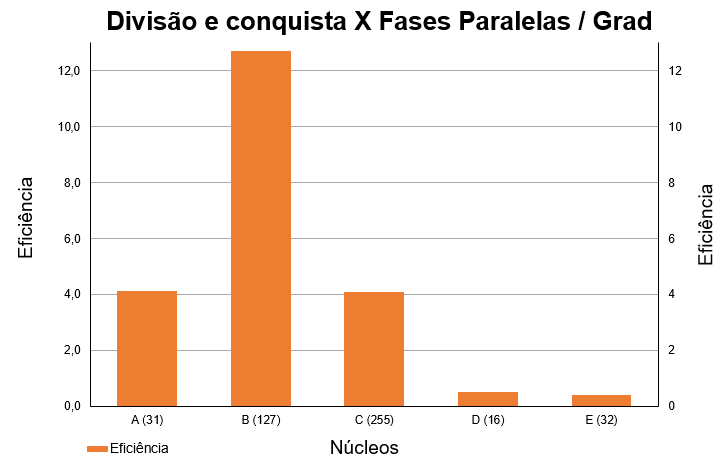
\includegraphics[width=9cm, height=5cm]{Capture.PNG}
            \vspace{-1.9em}
            \caption{Gráfico de eficiência comparando D\&C(A,B,C) com FP(D,E)}
            \vspace{-1.2em}
\end{figure}
\section{Observações Finais}
A utilização do algoritmo de fases paralelas se mostrou mais eficiente que a execução sequencial, como era esperado, porém, não foi o melhor algoritmo visto no decorrer da disciplina, ficando atrás dos outros dois processamentos paralelos abordados em aula: o mestre-escravo e o divisão e conquista. Obteve-se resultados razoáveis de speed-up e eficiência, entretanto esses também foram inferiores aos valores obtidos na execução dos outros algoritmos vistos. É importante analisar a diferença nos tempos medidos para as alterações da quantidade de elementos trocados entre os vetores para realizar a ordenação de maneira correta, sendo este o aspecto mais intrínseco do algoritmo.

\end{multicols*}

\newpage

\lstinputlisting[language=C++]{tpp3.c}

\end{document}
